\part{Problem, data and evaluation}
\section{Problem definition and dataset}
\subsection{Task and motivation}
The task is ten-class classification of a $28\times28$ grayscale image of an item of clothing. Given an input $x\in[0,1]^{1\times28\times28}$, a model returns ten logits $z=f_\theta(x)$. The predicted class is $\hat y=\arg\max_k z_k$. The five required Fashion-MNIST models are trained from scratch; no pretrained backbone or external training images are used for that comparison. Section~\ref{sec:garmentlab} describes a separate RGB extension with ImageNet initialization.

The analysis addresses three research questions:
\begin{enumerate}
\item \textbf{Representation:} How do pixel vectors, local feature maps, row sequences and patch tokens differ in classification errors, parameter count and measured computation under a shared data protocol?
\item \textbf{Recipe selection:} Which training recipes survive a bounded search, and how consistently do their paired-seed gains support the selection decision?
\item \textbf{Checkpoint objective:} How does selecting for class-wise F1 differ from selecting for probability loss along the same training trajectory?
\end{enumerate}
The original test comparison addresses fixed-checkpoint predictive performance. The subsequent studies examine duration, ablations and recipe selection on validation data. Their different evaluation roles are retained throughout the analysis.

Fashion-MNIST contains 60,000 official training images and 10,000 official test images, with ten balanced classes \cite{fashionmnist}. The official training images provide both training and validation data in this project. Each image is treated as one split unit. The class meanings are fixed by the dataset rather than inferred from file order.

\begin{center}
\small
\begin{tabular}{rlrr}
\toprule
Label & Class & Official train & Official test \\
\midrule
0 & T-shirt/top & 6,000 & 1,000 \\
1 & Trouser & 6,000 & 1,000 \\
2 & Pullover & 6,000 & 1,000 \\
3 & Dress & 6,000 & 1,000 \\
4 & Coat & 6,000 & 1,000 \\
5 & Sandal & 6,000 & 1,000 \\
6 & Shirt & 6,000 & 1,000 \\
7 & Sneaker & 6,000 & 1,000 \\
8 & Bag & 6,000 & 1,000 \\
9 & Ankle boot & 6,000 & 1,000 \\
\bottomrule
\end{tabular}
\end{center}
The dataset is distributed as compressed IDX image/label files by the Fashion-MNIST project under the MIT license: \url{https://github.com/zalandoresearch/fashion-mnist}. Raw-file checksums and a training-dataset fingerprint identify the downloaded data. A separate exact-pixel audit found zero duplicate groups among all 70,000 images, including zero cross-partition exact duplicates. That audit compares raw pixel equality; it does not rule out near-duplicates or visually related examples.\par

\subsection{Evidence layers}
The core analysis uses three completed studies with different purposes:
\begin{center}\small
\begin{tabularx}{\linewidth}{lrlX}\toprule
Study & Epochs & Checkpoint target & Evaluation role\\\midrule
Original & 20 & Minimum validation CE & Frozen checkpoints on official test; seed 42\\
Intermediate & 60 & Minimum validation CE & Duration and matched-seed ablations; seeds 42/43/44\\
OPT3 & 60 & Maximum validation F1 & Inner recipe selection, then final selected-validation estimates; seeds 42/43/44\\
\bottomrule\end{tabularx}\end{center}
Only the original study supplies official-test results. The later validation analyses reuse previously inspected data and describe optimization behavior rather than new blind-test generalization. This distinction prevents differences in evaluation split and checkpoint objective from being mistaken for a measured test improvement.

\bigskip
\section{EDA and preprocessing}

\begin{figure}[H]
\centering
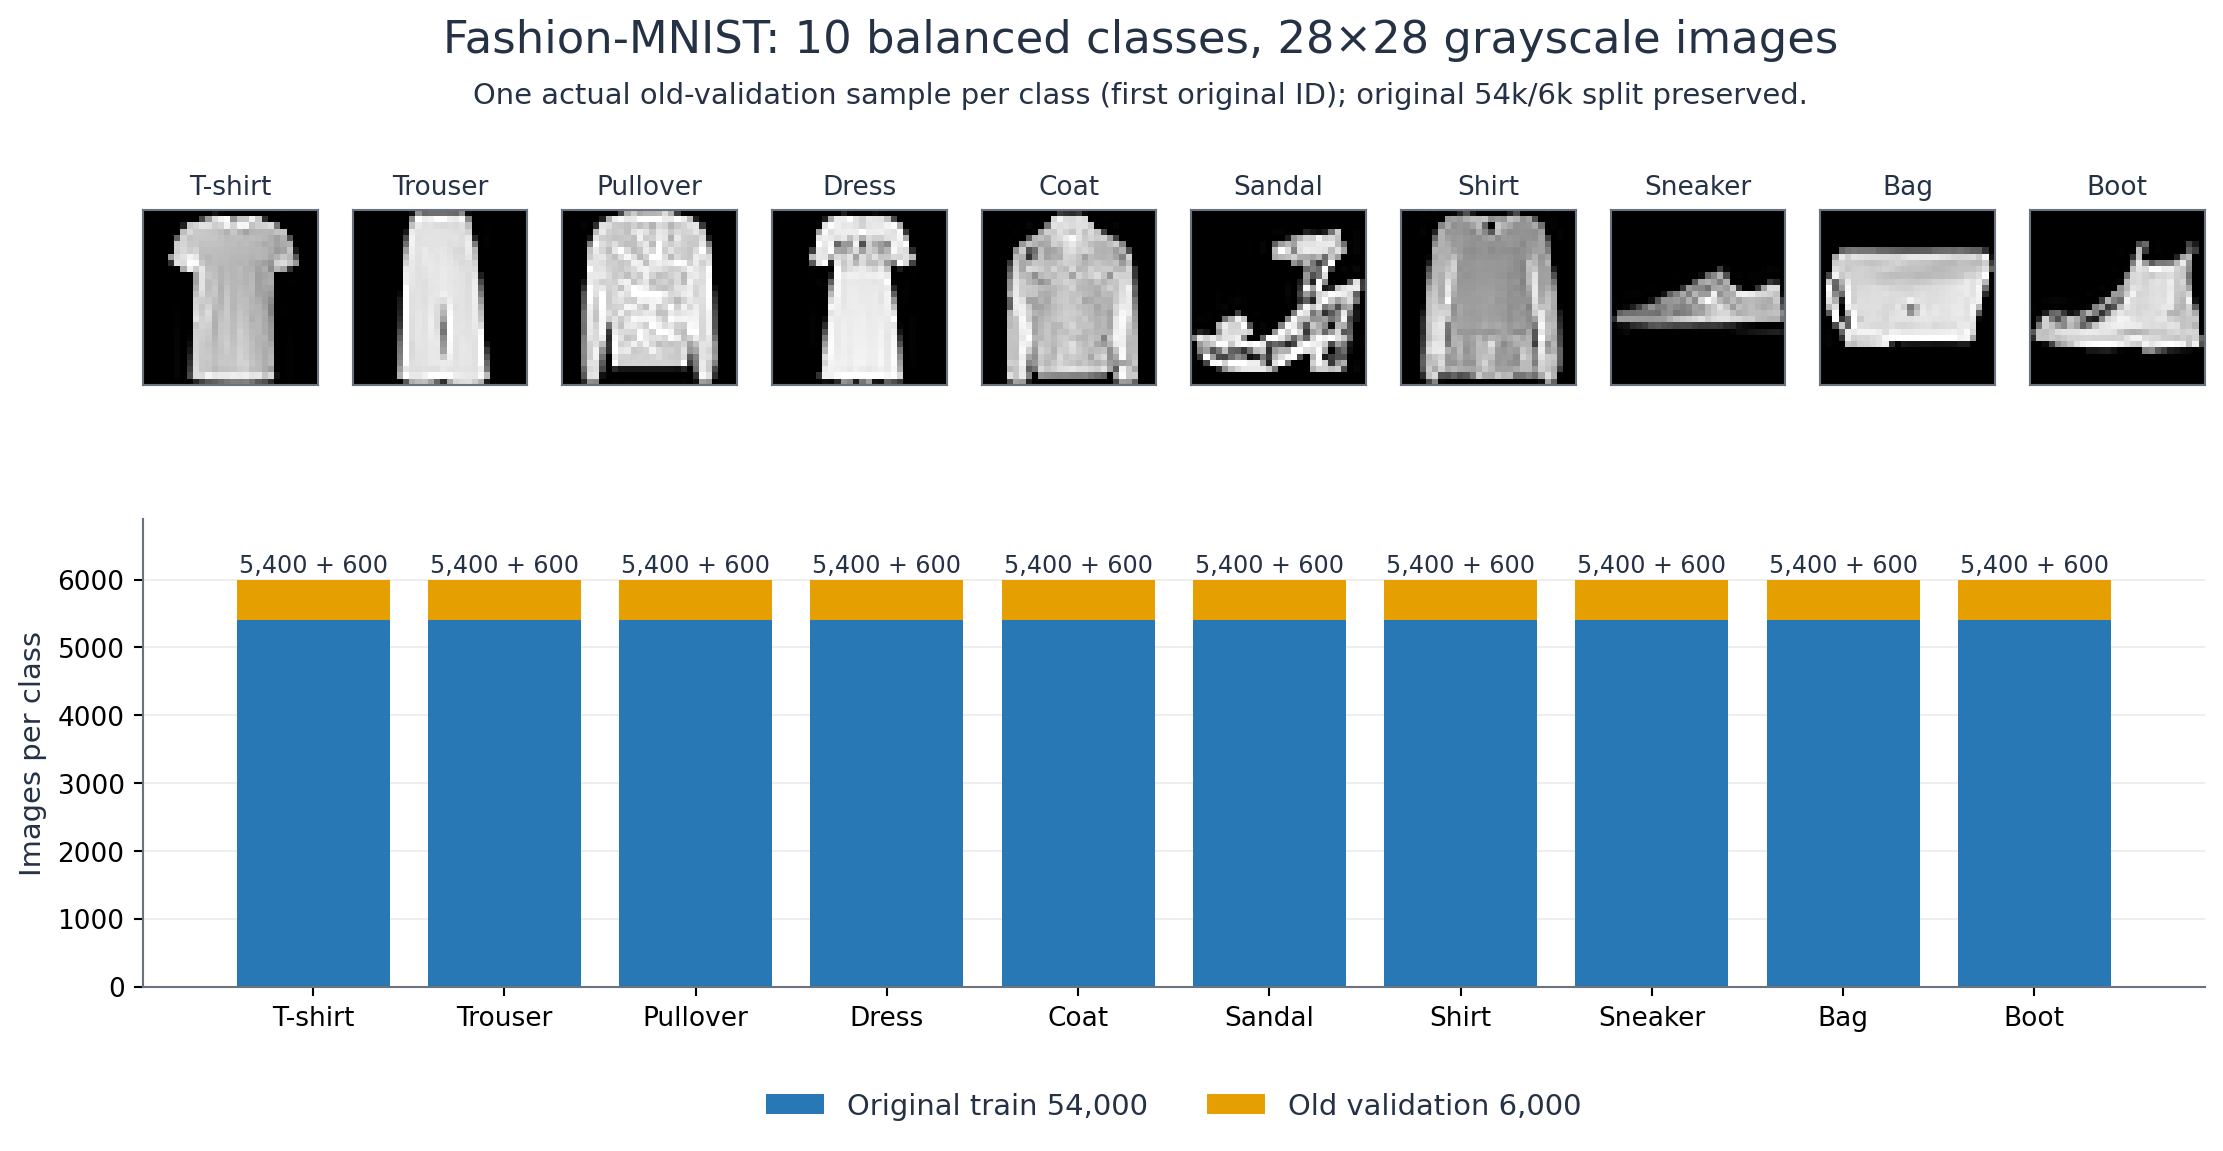
\includegraphics[width=\linewidth]{figures/dataset_overview.png}
\caption{Actual Fashion-MNIST samples and class counts from the preserved original split. The samples are the first old-validation ID in each true class; they are illustrative rather than randomly sampled.}
\label{fig:data}
\end{figure}
\subsection{Observed structure and ambiguity}
The data are balanced at the class level, but class difficulty is uneven. T-shirts, shirts, pullovers and coats often share grayscale outlines, whereas footwear and bags have more distinctive silhouettes in the displayed samples. Accuracy and macro-F1 are therefore complemented by class-level confusion rates. The sample grid motivates this analysis; the full predictions quantify its frequency.

At $28\times28$ pixels, color and fine texture are unavailable. Local edges and spatial arrangement motivate the CNN representation, while row and patch representations test alternative ways to encode context. Ambiguous thumbnails are retained with the supplied labels; visual ambiguity alone is insufficient evidence for relabeling.

\subsection{Input pipeline}
\begin{center}\small
\fbox{IDX images/labels}\ $\longrightarrow$\ \fbox{Saved split IDs}\ $\longrightarrow$\ \fbox{Float32 image tensors}\\[3mm]
\fbox{One of five models}\ $\longrightarrow$\ \fbox{Ten logits}\ $\longrightarrow$\ \fbox{CE for training; argmax for labels}
\end{center}
\texttt{ToTensor} converts unsigned pixel values from $[0,255]$ to float32 values in $[0,1]$. A batch has shape $B\times1\times28\times28$ and integer targets have shape $B$. The classification loss receives logits directly. Softmax is used conceptually to interpret class probabilities, not inserted before cross-entropy.

The recorded studies use no augmentation, channel-wise standardization, oversampling or pretrained features. A seeded generator shuffles training batches; validation uses a fixed order. Both loaders retain the short final batch.

During training, each minibatch performs gradient reset, forward propagation, cross-entropy evaluation, backpropagation, gradient-norm clipping and an optimizer update. Validation runs in evaluation mode with gradients disabled and does not update parameters. Epoch CE is sample-weighted,
\[
\mathrm{CE}_{\mathrm{epoch}}=\frac{\sum_b n_b\,\mathrm{CE}_b}{\sum_b n_b},
\]
so a short final batch has its correct contribution. Accuracy and macro-F1 are computed from the complete epoch confusion matrix, equivalently all epoch predictions, rather than averaging minibatch F1 values. Saved IDs connect those predictions to the original dataset images.

\bigskip
\section{Evaluation design}
\subsection{Preserved and nested partitions}
The original split uses split seed 42 and is stratified. Its sample IDs are retained throughout all studies. The final search creates one additional stratified split inside the original 54,000 training IDs, using inner split seed 20261022. All families use identical IDs at a given phase.

\begin{center}
\small
\begin{tabular}{lrrl}
\toprule
Partition & Images & Images/class & Role in final study \\
\midrule
Original train & 54,000 & 5,400 & Parent set for search; final training \\
Old validation & 6,000 & 600 & Final checkpoint selection \\
Inner train & 48,600 & 4,860 & Discovery and confirmation training \\
Inner validation & 5,400 & 540 & Recipe and checkpoint selection \\
Official test & 10,000 & 1,000 & Historical frozen results only \\
\bottomrule
\end{tabular}
\end{center}
Inner train and inner validation are disjoint and together recover the original training set. Neither contains old-validation IDs. Final training uses the original 54,000 images, with old validation still excluded from gradient updates. Each fit starts from a fresh seeded initialization. This keeps the inner-validation images outside the weight-update history of every search candidate.

\subsection{Metrics and checkpoint rules}
For a validation set of $N$ images, accuracy is $N^{-1}\sum_i\mathbf{1}[\hat y_i=y_i]$. For class $k$,
\[
F_{1,k}=\frac{2TP_k}{2TP_k+FP_k+FN_k},\qquad
F_{1,\mathrm{macro}}=\frac{1}{10}\sum_{k=0}^{9}F_{1,k}.
\]
Cross-entropy is $\mathrm{CE}=-N^{-1}\sum_i\log p_\theta(y_i\mid x_i)$. It is sensitive to the probability assigned to the true label; accuracy and macro-F1 depend on predicted classes. A later checkpoint may therefore improve F1 while worsening CE.

The original and intermediate studies retain the minimum-validation-CE checkpoint, taking the earliest epoch on an exact tie. Final OPT3 uses maximum validation macro-F1; exact F1 ties prefer lower CE, followed by the earlier epoch. These rules apply to every family within their respective study. Best-CE checkpoints are also retained as a secondary diagnostic. The OPT3 rule was fixed before the search began; the later study remains exploratory because the earlier test results were already known.

\subsection{Meaning of the reported variation}
For final seeds $s\in\{42,43,44\}$, the report gives the arithmetic mean and sample standard deviation, with denominator $n-1$. These quantify training-seed variation conditional on the fixed, selected validation set. Image-sampling uncertainty, split variation and deployment shift are outside this SD; the three runs are used descriptively rather than as a significance test.

\clearpage
\part{Models and optimization}
\section{Five model families}
\subsection{Architecture and parameter summary}
All models output $B\times10$ logits. Architecture sizes are held fixed in the search. Dropout changes stochastic regularization without adding parameters; schedule changes do not add parameters either.

\begin{center}
\small
\begin{tabular}{llr}
\toprule
Family & Main representation & Trainable parameters \\
\midrule
Linear & $784\rightarrow10$ & 7,850 \\
MLP & $784\rightarrow256\rightarrow10$ & 203,530 \\
CNN & 3 convolutions, channels $32/64/128$ & 93,962 \\
GRU & 28 steps, input 28, hidden 128 & 61,962 \\
Transformer & 49 patches, width 128, 2 layers & 274,954 \\
\bottomrule
\end{tabular}
\end{center}
\subsection{Linear classifier}
The image is flattened to 784 features and mapped by $z=Wx+b$ to ten logits. The parameter count is $784\cdot10+10=7,850$. Its decision boundaries are linear in pixel space, providing a low-cost reference for the value of nonlinear and spatial representations.

\subsection{MLP}
The MLP applies a 256-unit affine layer, ReLU and a ten-unit output layer:
\[
z=W_2\,\mathrm{ReLU}(W_1\,\mathrm{vec}(x)+b_1)+b_2.
\]
Its parameter count is $(784\cdot256+256)+(256\cdot10+10)=203,530$. ReLU makes the mapping nonlinear, but flattening removes an explicit local spatial bias. The final selected C7 recipe applies dropout $p=0.2$ to the hidden representation before the output layer.

\subsection{Custom CNN}
Three $3\times3$ convolutions use stride 1 and padding 1. ReLU follows each convolution. The first two blocks include $2\times2$ max pooling. The spatial shapes are
\[
\begin{split}
B\times1\times28\times28\rightarrow B\times32\times28\times28
\rightarrow B\times32\times14\times14\\
\rightarrow B\times64\times14\times14\rightarrow B\times64\times7\times7
\rightarrow B\times128\times7\times7.
\end{split}
\]
Global average pooling produces $B\times128$, followed by dropout and a ten-unit head. Convolutions contribute 320, 18,496 and 73,856 parameters; the head contributes 1,290, for 93,962 total. Local receptive fields and shared filters reduce the number of parameters needed to detect repeated spatial patterns. Pooling and global averaging reduce spatial detail while providing some tolerance to position changes. C5 retains the architecture and uses head dropout 0.3.

\clearpage
\subsection{Row-wise GRU}
Each image is a sequence of 28 rows, each containing 28 pixel values. The input becomes $B\times28\times28$. A one-layer, unidirectional GRU with hidden size 128 returns a final hidden state $h_{28}\in\mathbb{R}^{B\times128}$, followed by a linear classifier. The update gate controls how much of the previous hidden state is retained, while the reset gate controls its contribution to the candidate state \cite{gru}. In the PyTorch implementation,
\[
\begin{aligned}
r_t&=\sigma(W_{ir}x_t+b_{ir}+W_{hr}h_{t-1}+b_{hr}),\\
z_t&=\sigma(W_{iz}x_t+b_{iz}+W_{hz}h_{t-1}+b_{hz}),\\
\widetilde h_t&=\tanh\!\left(W_{in}x_t+b_{in}+r_t\odot(W_{hn}h_{t-1}+b_{hn})\right),\\
h_t&=(1-z_t)\odot\widetilde h_t+z_t\odot h_{t-1}.
\end{aligned}
\]
Here $x_t\in\mathbb R^{28}$ and $h_t,r_t,z_t\in\mathbb R^{128}$. The reset gate is applied after the hidden-state affine transform, matching the implemented library operation.\footnote{PyTorch 2.11 GRU definition: \url{https://docs.pytorch.org/docs/2.11/generated/torch.nn.GRU.html}.}

The row representation imposes an ordering on spatial data. It can summarize dependencies across image rows, but introduces directional bias and sequential computation. The matched row-versus-column ablation examines the effect of this ordering for the fixed architecture and training setup.

The parameter count is
\[
3(128)(28)+3(128)(128)+2(3)(128)+(128)(10)+10=61,962.
\]
For one recurrent layer, PyTorch's built-in GRU dropout between layers is inactive. The optimization implementation therefore provides explicit optional dropout on the final hidden state. The selected C1 recipe uses no external head dropout and retains the row representation.

\subsection{Patch Transformer}
A stride 4, kernel 4 convolution embeds non-overlapping patches. The $28\times28$ image yields $7\times7=49$ tokens, each of dimension 128. Learned position embeddings have shape $1\times49\times128$. Two encoder layers each use four attention heads, a 256-wide feed-forward block, ReLU, residual connections, layer normalization and dropout. Attention uses
\[
\mathrm{Attention}(Q,K,V)=\mathrm{softmax}\left(\frac{QK^\top}{\sqrt{d_k}}\right)V,
\qquad d_k=128/4=32.
\]
Within each head, $Q$, $K$ and $V$ are learned projections of the 49 position-enriched token features, each with shape $B\times49\times32$. Attention weights relate every query patch to all key patches; the weighted values form contextual token representations. Four head outputs are concatenated and projected back to width 128. After the two encoder layers, mean pooling over the 49 tokens, LayerNorm and a ten-class linear head produce the logits. The from-scratch encoder uses no class token and has 274,954 trainable parameters \cite{attention}.

The model can relate distant patches in one attention layer, but learns both feature extraction and spatial use from this small dataset. The search includes an independently initialized encoder probe because the legacy encoder layers begin with equal initial values while remaining distinct parameters. The selected C1 recipe retains legacy initialization and uses warmup plus cosine decay. The initialization probe is one candidate comparison within this search, rather than a general conclusion about encoder initialization.

\subsection{Training objective and optimizers}
All five families minimize hard-label cross-entropy on minibatches of 128. Gradient norm clipping uses threshold 1. Inputs and model parameters are float32, without mixed-precision scaling. Linear and MLP use Adam \cite{adam}; CNN, GRU and Transformer use AdamW \cite{adamw}. Optimizer type and model size remain fixed during the final search. Adam applies the configured decay within its gradient-based update, whereas AdamW decouples decay from the adaptive gradient step. Equal numeric coefficients therefore do not define identical regularization across these optimizer families.

\clearpage
\section{Optimization protocol}
\subsection{Question, search space and budget}
The final study asks whether training recipes improve within fixed model families. It uses a seeded, finite random search with controlled probes, rather than a full Cartesian grid or Bayesian adaptation. Optuna's RandomSampler is used to generate candidate values before observing objective scores \cite{optuna}. The candidate manifest is fixed, and no performance-based pruning replaces a weak candidate.

Linear has four candidates; the other four families each have eight. Candidate C0 is the original anchor. C1 changes the learning-rate schedule. C2 is a targeted probe for each nonlinear family: MLP/GRU external head dropout, CNN weight decay, or independent Transformer encoder initialization. Remaining candidates sample learning rate, weight decay and applicable dropout. Constant and scheduled learning rates are balanced within each family: 2/2 for Linear and 4/4 otherwise.

\begin{center}
\small
\begin{tabular}{lcll}
\toprule
Family & Candidates & LR range & Applicable dropout \\
\midrule
Linear & 4 & $3\times10^{-4}$--$3\times10^{-3}$ & None \\
MLP & 8 & $3\times10^{-4}$--$3\times10^{-3}$ & Hidden $0/0.1/0.2/0.3$ \\
CNN & 8 & $3\times10^{-4}$--$3\times10^{-3}$ & Head $0/0.1/0.2/0.3$ \\
GRU & 8 & $2\times10^{-4}$--$2\times10^{-3}$ & External head $0/0.1/0.2/0.3$ \\
Transformer & 8 & $10^{-4}$--$10^{-3}$ & Encoder $0.05/0.1/0.2/0.3$ \\
\bottomrule
\end{tabular}
\end{center}
Learning rates are sampled on a log scale. Sampled weight decay is one of $0,10^{-5},10^{-4},10^{-3}$. Controlled anchors/probes may retain the original value outside a sampled dropout range; the realized manifest is the authoritative candidate list in Appendix\ \ref{app:recipes}. There are only 36 discovery points across all five families, so the study cannot establish global hyperparameter optimality.

\subsection{Schedule and duration}
Every task completes 60 epochs. Constant schedules keep the configured learning rate. Cosine schedules decay to 5\% of the initial value; the Transformer scheduled probe combines five warmup epochs with cosine decay. The schedule follows optimizer-update counts and resumes from the saved update state. There are no cosine restarts. Inner fits use 380 updates per epoch, while final fits use 422, because $\lceil48,600/128\rceil=380$ and $\lceil54,000/128\rceil=422$.

The final stage trains on all 54,000 original training images for 60 epochs and retains the best checkpoint on the old 6,000-image validation set. Training completes the full budget; early stopping is not used. The selected epoch and the total executed epochs are recorded separately.

\clearpage
\subsection{Discovery, confirmation and final fits}
\begin{enumerate}
\item \textbf{Discovery:} The 36 candidates were trained with seed 101 on 48,600 inner-training images. Inner-validation macro-F1 selected the checkpoint within each fit and the best non-anchor challenger for each family. Scores within absolute $10^{-6}$ favored the lowest candidate ID.
\item \textbf{Additional confirmation:} C0 and the challenger for each family were trained with seed 202, giving 10 new fits. The decision used mean selected inner macro-F1 over seeds 101 and 202. A challenger was retained only when it exceeded the anchor mean by more than $10^{-6}$; otherwise C0 was retained.
\item \textbf{Final study:} The selected recipe for each family was trained from scratch with seeds 42,43 and 44 on the original 54,000 images. The old 6,000-image validation set selected the F1 checkpoint. These 15 completed fits form the final exploratory summary.
\end{enumerate}
The total is $36+10+15=61$ completed tasks and $61\cdot60=3,660$ model-epochs. Seed 101 is also used to discover the challenger. Thus, there is \emph{one fresh confirmation seed}, not two independently held-out confirmation runs. A positive mean across the two seeds is the locked decision rule, not a significance test.

\subsection{Controls and recovery}
Candidate configurations, effective hashes, source snapshots and split IDs bind a task to its intended recipe. Completed tasks preserve F1- and CE-selected checkpoints, predictions and a full 60-epoch history. Task transactions retain optimizer/RNG/loader state and checkpoint-selection state for recovery. A resumed task retains the same identity and random-state history; it is not counted as another independent seed.

All 61 recorded task attempts completed without an error. Software checks and experimental measurements are recorded separately.

\subsection{Selection scope}
The inner validation set is used for both checkpoint and recipe selection. The final old-validation set is also used to select final checkpoints. Its final score is consequently a selected validation estimate. The 15-fit OPT3 final stage did not train fresh C0 anchors alongside its selected recipes. That phase cannot isolate the effect of the recipe changes. Section~\ref{sec:matched-followup} supplies the later matched controls. Differences from older CE-selected baselines combine recipe changes, selection rules and potentially implementation/runtime effects.

\clearpage
\part{Results and interpretation}
\section{Original test study and intermediate evidence}
\subsection{Frozen official-test results}
Table\ \ref{tab:test} reports the original 20-epoch, seed 42 checkpoints evaluated on the 10,000-image official test. The checkpoints were selected by validation CE before the test evaluation. The later OPT3 checkpoints are evaluated only on validation, so this table remains the report's official-test comparison.
\begin{table}[H]\centering
\caption{Historical official-test results: original 20-epoch study, one training seed.}\label{tab:test}

\begin{center}
\small
\begin{tabular}{lrrrr}
\toprule
Model & Test accuracy(\%) & Test macro-F1(\%) & Parameters & Epoch \\
\midrule
Linear & 84.68 & 84.590 & 7,850 & 18 \\
MLP & 88.74 & 88.699 & 203,530 & 20 \\
CNN & 89.59 & 89.524 & 93,962 & 20 \\
GRU & 89.14 & 89.145 & 61,962 & 18 \\
Transformer & 88.94 & 88.829 & 274,954 & 20 \\
\bottomrule
\end{tabular}
\end{center}
\end{table}
The CNN has the highest recorded test accuracy, 89.59\%, exceeding the linear classifier by 4.91 percentage points. This is a fixed-budget, single-seed comparison. Its test estimates and the later selected-validation estimates answer different evaluation questions.

\subsection{Why extend beyond 20 epochs?}
The intermediate study uses seeds 42,43 and 44, best-CE selection, and a 60-epoch budget. For the CNN, best-through 60 minus best-through 20 improves validation accuracy by 2.417 percentage points on average, with sample SD 0.342. The MLP's best-CE F1 does not improve under that extension. More epochs therefore do not help every model equally.

The same intermediate study tests three ablations. Table\ \ref{tab:ablations} gives variant-minus-baseline F1 differences at 60 epochs. These are matched-seed validation comparisons under the earlier CE-selection protocol, separate from final OPT3.
\begin{table}[H]\centering\caption{Intermediate 60-epoch ablations; macro-F1 difference in percentage points, mean $\pm$sample SD over three matched seeds.}\label{tab:ablations}

\begin{center}
\small
\begin{tabular}{lr}
\toprule
Variant minus baseline & Macro-F1 delta(pp) \\
\midrule
cnn\_no\_dropout & $-0.069 \pm 0.155$ \\
gru\_columns & $-0.570 \pm 0.216$ \\
transformer\_no\_position & $-3.903 \pm 0.148$ \\
\bottomrule
\end{tabular}
\end{center}
\end{table}
CNN dropout removal has mixed-seed effects. Column scanning lowers GRU F1 on all three seeds. Removing Transformer positions also removes 6,272 parameters, so this probe changes capacity as well as position information.

\clearpage
\section{Final OPT3 validation results}
The selected recipes are Linear C1, MLP C7, CNN C5, GRU C1 and Transformer C1. All final fits use 60 epochs and the same preserved 54k/6k partition. Table\ \ref{tab:final} summarizes the F1-selected checkpoints over three training seeds. Accuracy/F1 are expressed as percentages; SD is in percentage points.
\begin{table}[H]\centering\caption{Final exploratory validation results; three seeds, sample SD.}\label{tab:final}

\begin{center}
\small
\begin{tabular}{lrrr}
\toprule
Model/recipe & Accuracy(\%) & Macro-F1(\%) & CE \\
\midrule
Linear / C1 & $86.856 \pm 0.010$ & $86.851 \pm 0.024$ & $0.3790 \pm 0.0009$ \\
MLP / C7 & $91.439 \pm 0.167$ & $91.448 \pm 0.153$ & $0.2630 \pm 0.0012$ \\
CNN / C5 & $93.278 \pm 0.059$ & $93.308 \pm 0.027$ & $0.1915 \pm 0.0003$ \\
GRU / C1 & $91.400 \pm 0.328$ & $91.367 \pm 0.376$ & $0.2748 \pm 0.0137$ \\
Transformer / C1 & $91.433 \pm 0.120$ & $91.431 \pm 0.096$ & $0.3092 \pm 0.0177$ \\
\bottomrule
\end{tabular}
\end{center}
\end{table}
\begin{figure}[H]
\centering
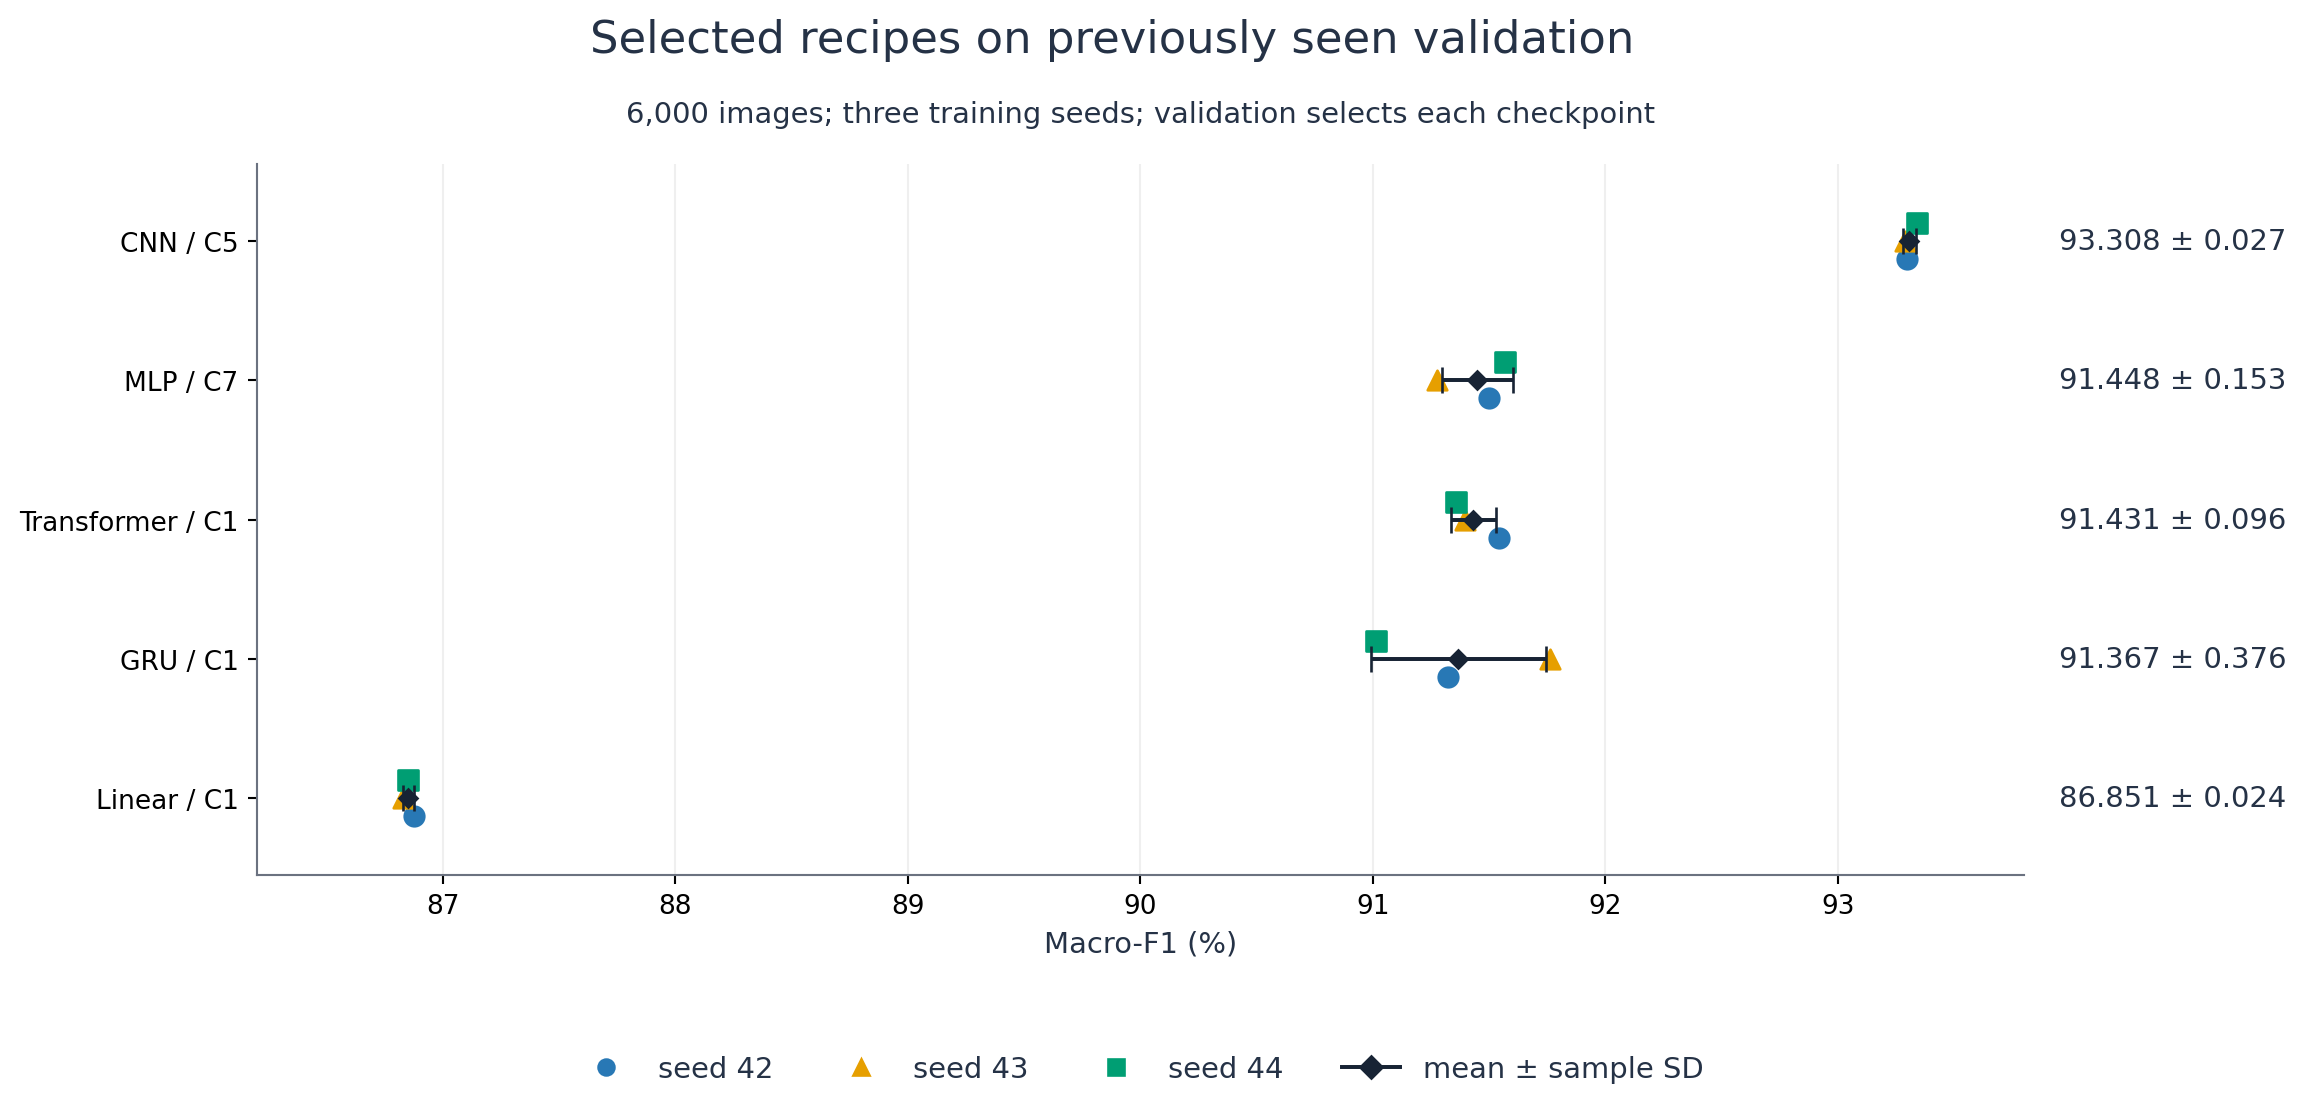
\includegraphics[width=\linewidth]{figures/final_f1_seeds.png}
\caption{Final old-validation macro-F1: individual seeds, mean and sample SD. Every point uses a checkpoint selected on these same 6,000 images. Small seed variation does not remove selection bias.}
\label{fig:final}
\end{figure}
CNN has the highest final validation mean. MLP and Transformer means are close, while GRU has greater seed variation. The ranking is conditional on Fashion-MNIST, the preserved split, the candidate space and the checkpoint-selection rule. The per-seed values are retained in Appendix\ \ref{app:seeds}.

\clearpage
\section{Search behavior and confirmation}
\subsection{Discovery coverage}

\begin{figure}[H]
\centering
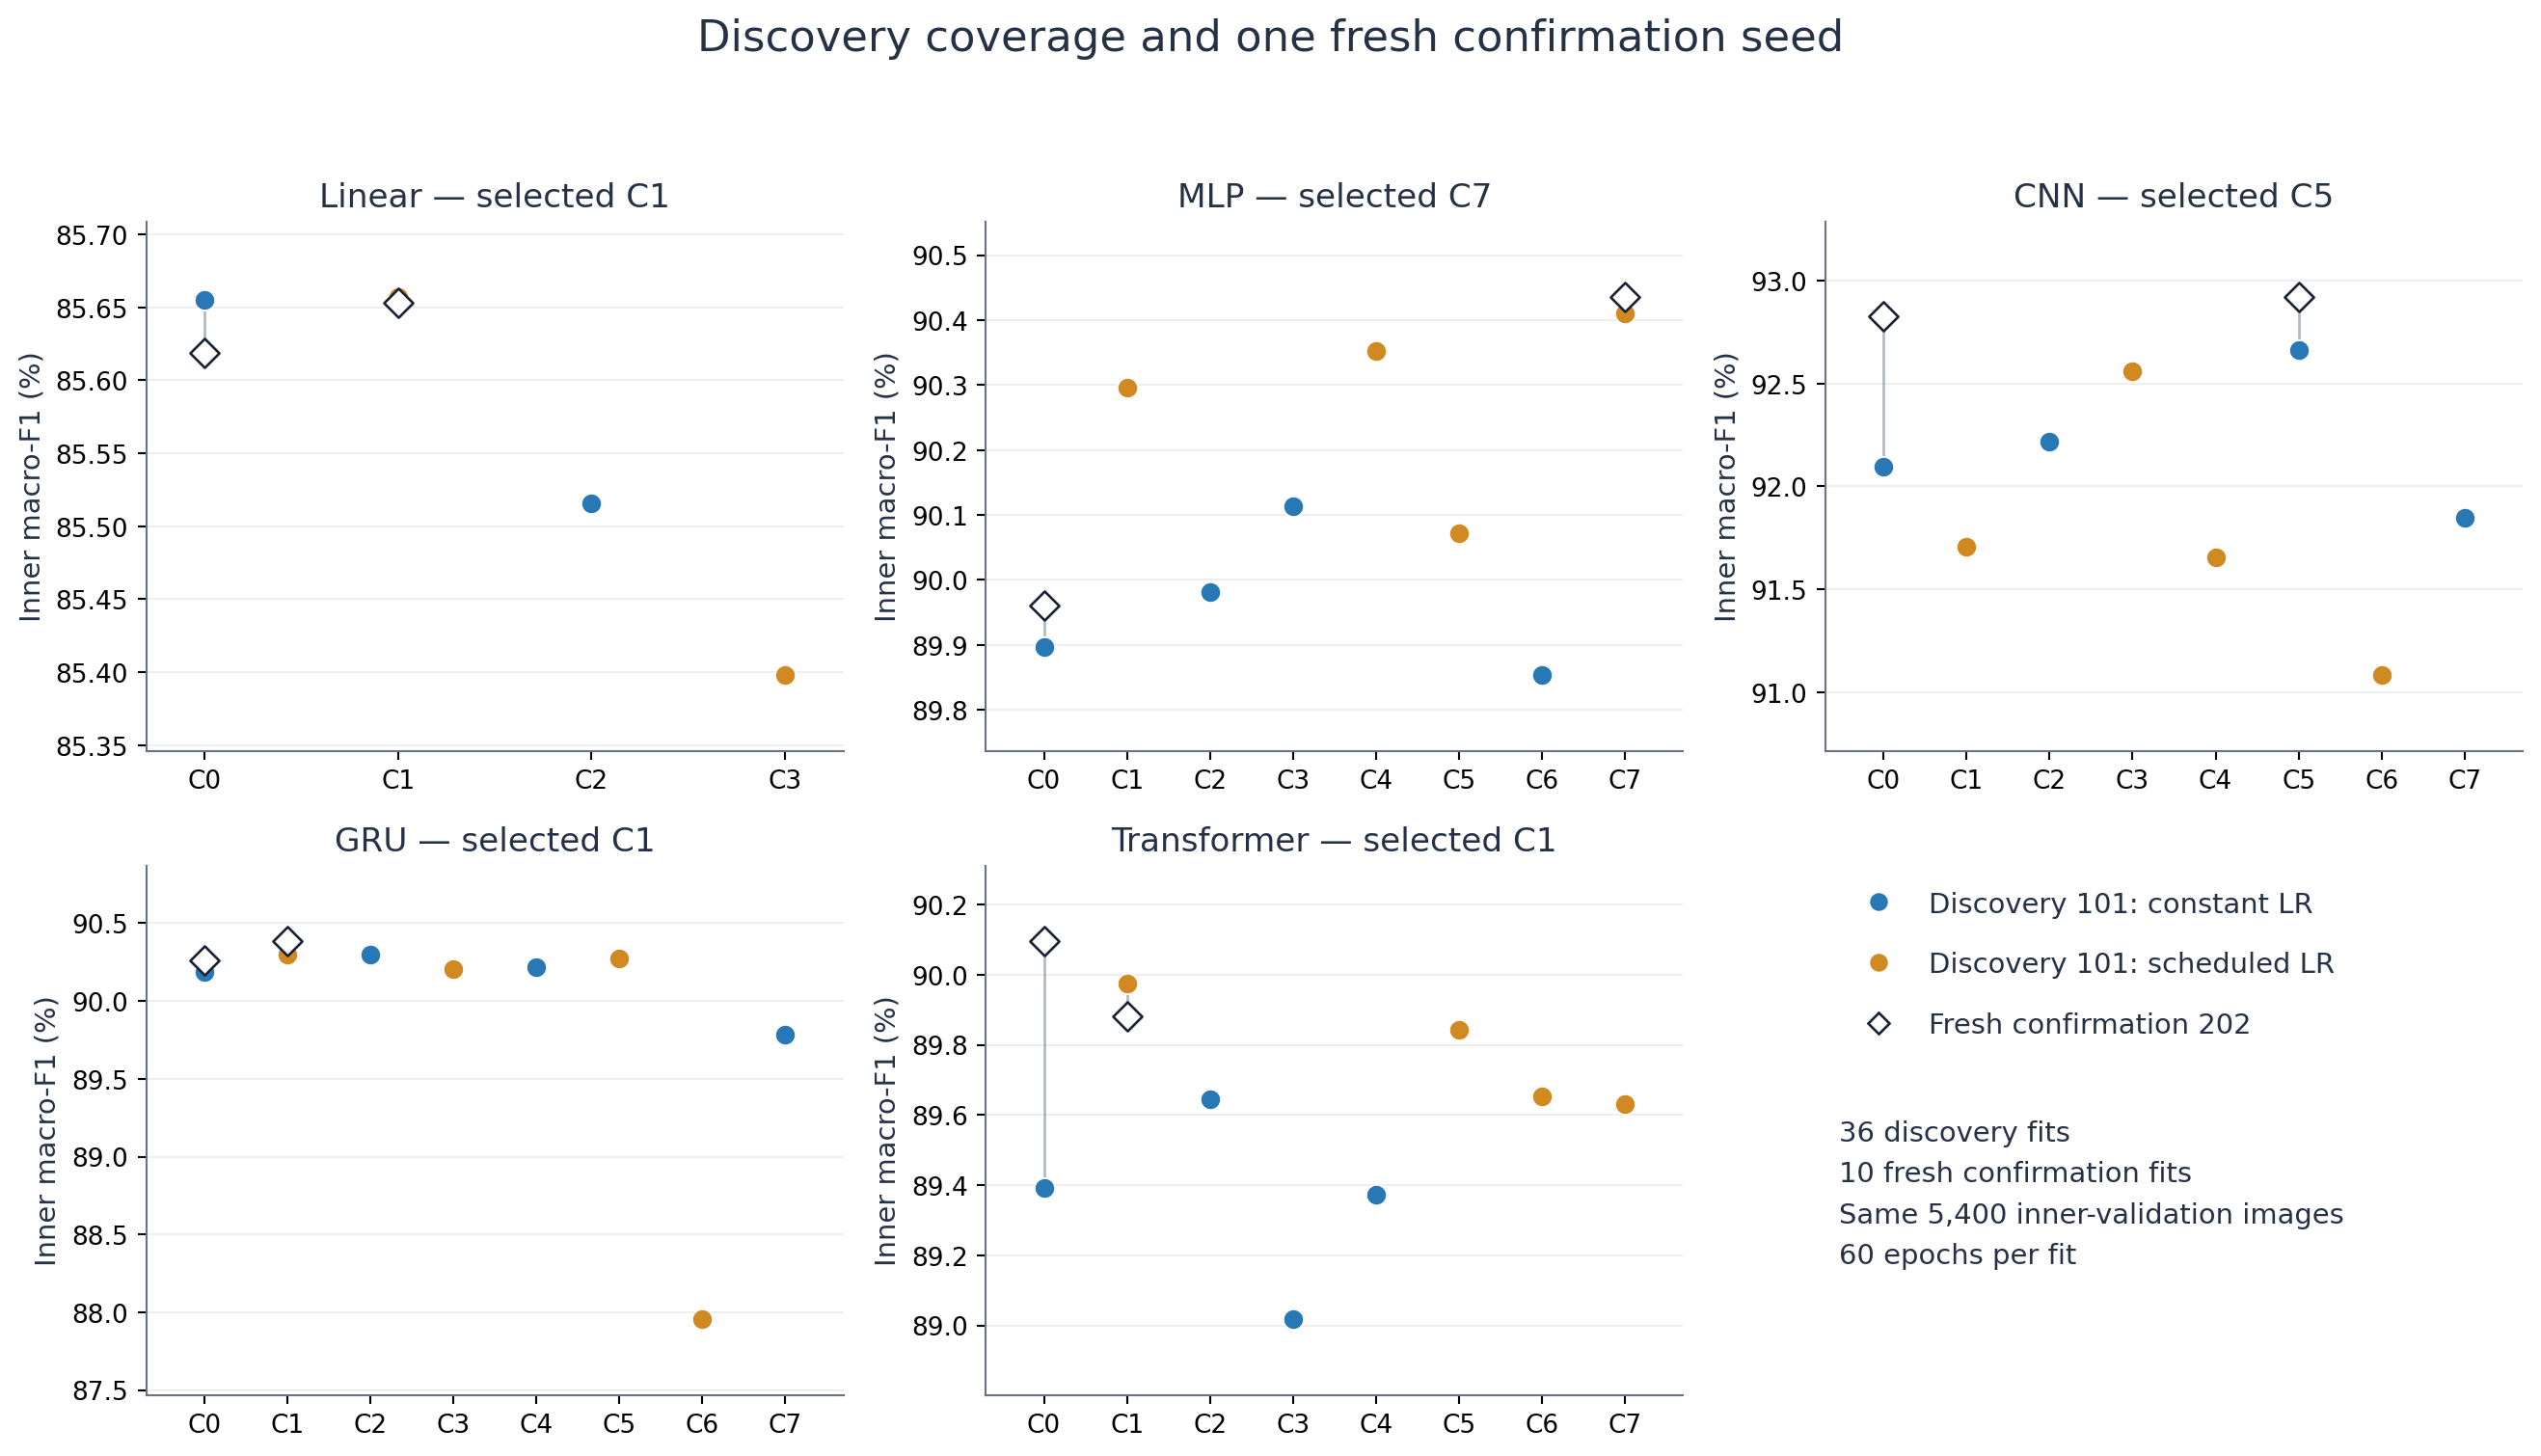
\includegraphics[width=\linewidth]{figures/discovery_confirmation.png}
\caption{All 36 discovery candidates and the 10 additional confirmation fits. Filled circles show seed 101; open diamonds show seed 202 for C0 and the selected challenger. Each panel uses the same inner-validation set but its own vertical scale.}
\label{fig:search}
\end{figure}
Several simple schedule probes survive the search: Linear, GRU and Transformer select C1. MLP selects C7, which combines cosine decay, learning rate approximately$1.010\times10^{-3}$, weight decay$10^{-5}$ and hidden dropout 0.2. CNN selects C5, a constant-LR recipe with learning rate approximately$1.438\times10^{-3}$, weight decay$10^{-4}$ and dropout 0.3.

These are recipe-level observations. The random candidates change multiple factors, so the MLP/CNN result does not identify a single responsible ingredient. The Transformer C1 probe combines warmup and cosine decay; its comparison does not isolate the effect of cosine alone. With eight candidates per nonlinear family, conclusions concern the realized recipes rather than global hyperparameter optima.

\clearpage
\subsection{Paired margins and one fresh seed}

\begin{figure}[H]
\centering
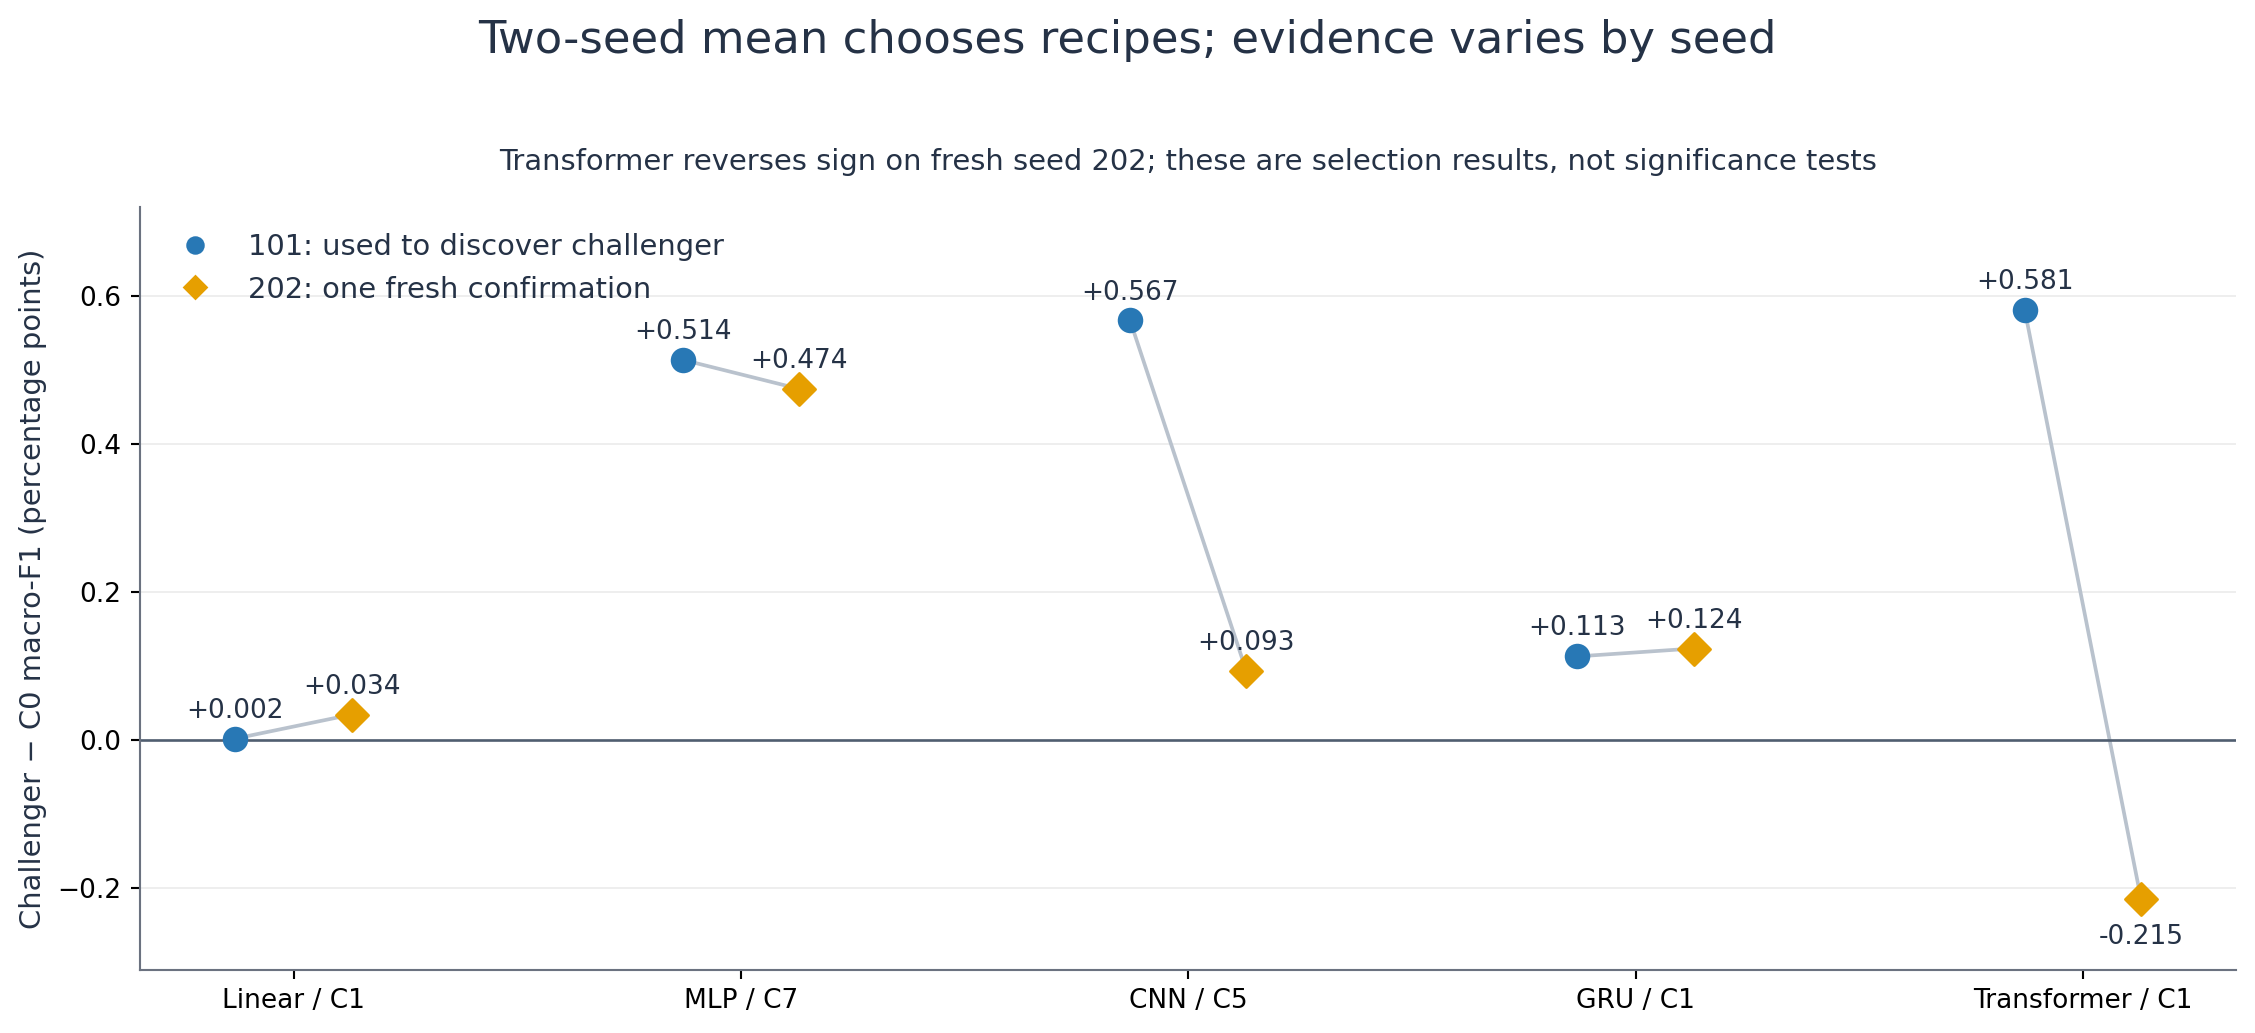
\includegraphics[width=\linewidth]{figures/paired_confirmation_deltas.png}
\caption{Challenger-minus-C0 F1 differences on the two matched inner seeds. Seed 101 already participated in discovery; seed 202 is the one fresh confirmation. Transformer changes sign, while the Linear difference is small.}
\label{fig:paired}
\end{figure}
\begin{center}
\small
\begin{tabular}{lcrrr}
\toprule
Family & Challenger & Seed 101(pp) & Seed 202(pp) & Mean(pp) \\
\midrule
Linear & C1 & +0.0020 & +0.0344 & +0.0182 \\
MLP & C7 & +0.5136 & +0.4743 & +0.4940 \\
CNN & C5 & +0.5668 & +0.0930 & +0.3299 \\
GRU & C1 & +0.1130 & +0.1236 & +0.1183 \\
Transformer & C1 & +0.5812 & -0.2146 & +0.1833 \\
\bottomrule
\end{tabular}
\end{center}
MLP C7 improves by about 0.514 and 0.474 percentage points on the two seeds. CNN C5 has a larger discovery gain than fresh-seed gain. Linear C1 clears the decision threshold but its mean gain is only about 0.018 percentage points. The Transformer gains 0.581 points on seed 101 and loses 0.215 on seed 202. Its positive two-seed mean selects C1 under the locked rule, while the mixed signs limit confidence that the change consistently improves this family.

The discovery seed's selected challenger is subject to selection bias because it was chosen from several alternatives. The second seed reduces dependence on a single lucky fit, but does not create a new data split. The individual paired margins expose the consistency and scale of the selection evidence.

\clearpage
\section{Learning dynamics and checkpoint choice}

\begin{figure}[H]
\centering
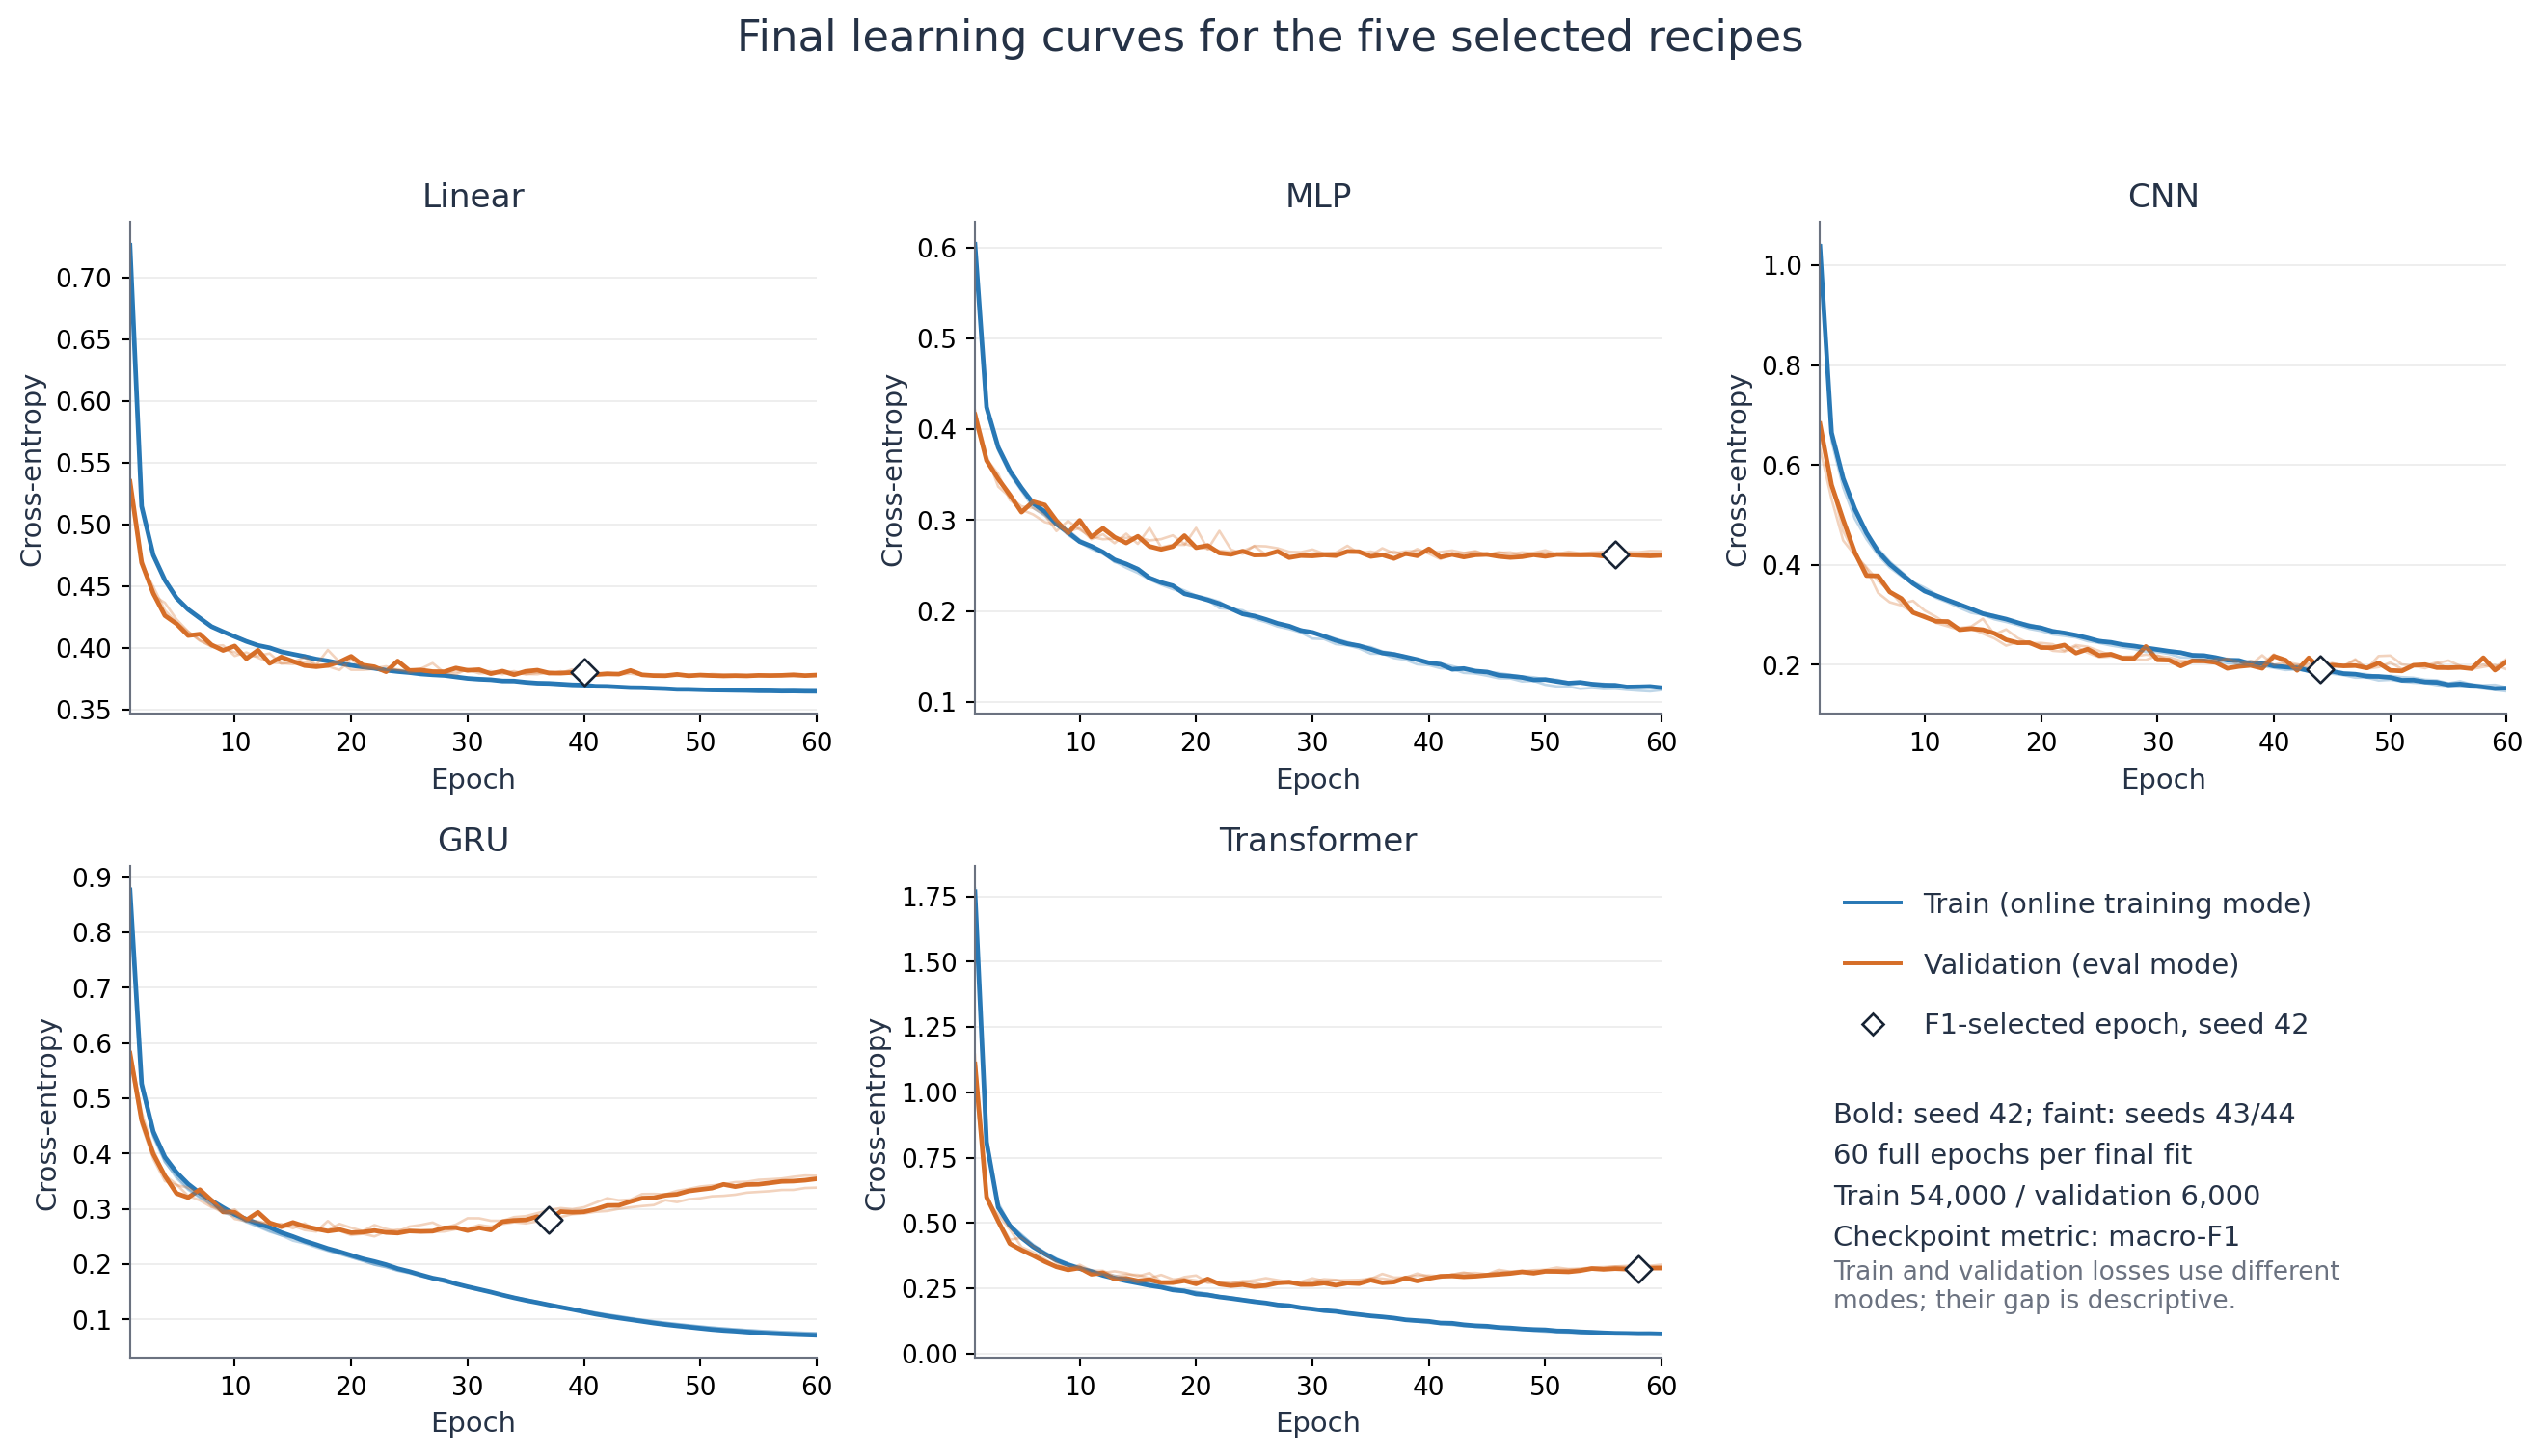
\includegraphics[width=\linewidth]{figures/learning_curves.png}
\caption{Actual unsmoothed final learning curves. Bold lines are seed 42; faint lines are seeds 43/44. Diamonds identify the seed 42 F1-selected epoch. Train loss is an online training-mode measure, whereas validation uses evaluation mode.}
\label{fig:curves}
\end{figure}
The CNN continues to learn useful representations late in training, although its validation CE fluctuates. MLP C7 reaches a comparatively flat validation-CE region while training loss continues downward. GRU and Transformer show increasing validation CE late in training even though some later epochs can still have competitive F1. CE deterioration diagnoses worsening probability loss, not necessarily worsening classification at every later epoch.

For CNN C5, seed 42, the F1 checkpoint is epoch 44: F1=0.932954 and CE=0.191585. The CE checkpoint is epoch 51: F1=0.932818 and CE=0.187897. Epoch 60 has F1=0.926353. Thus, choosing the last epoch would lose F1 in this particular fit, while minimum CE and maximum F1 select different valid checkpoints. The example demonstrates an objective trade-off along one trajectory: class-wise decision quality and true-label probability loss need not select the same epoch.

The train--validation gap cannot be interpreted as a perfectly matched measurement of generalization because train metrics use dropout and evolving weights during the epoch. Validation is measured after the epoch with dropout disabled. The upward validation-CE trend remains observable independently of that mode difference.

\clearpage
\section{Error analysis}
\subsection{CNN confusion structure}

\begin{figure}[H]
\centering
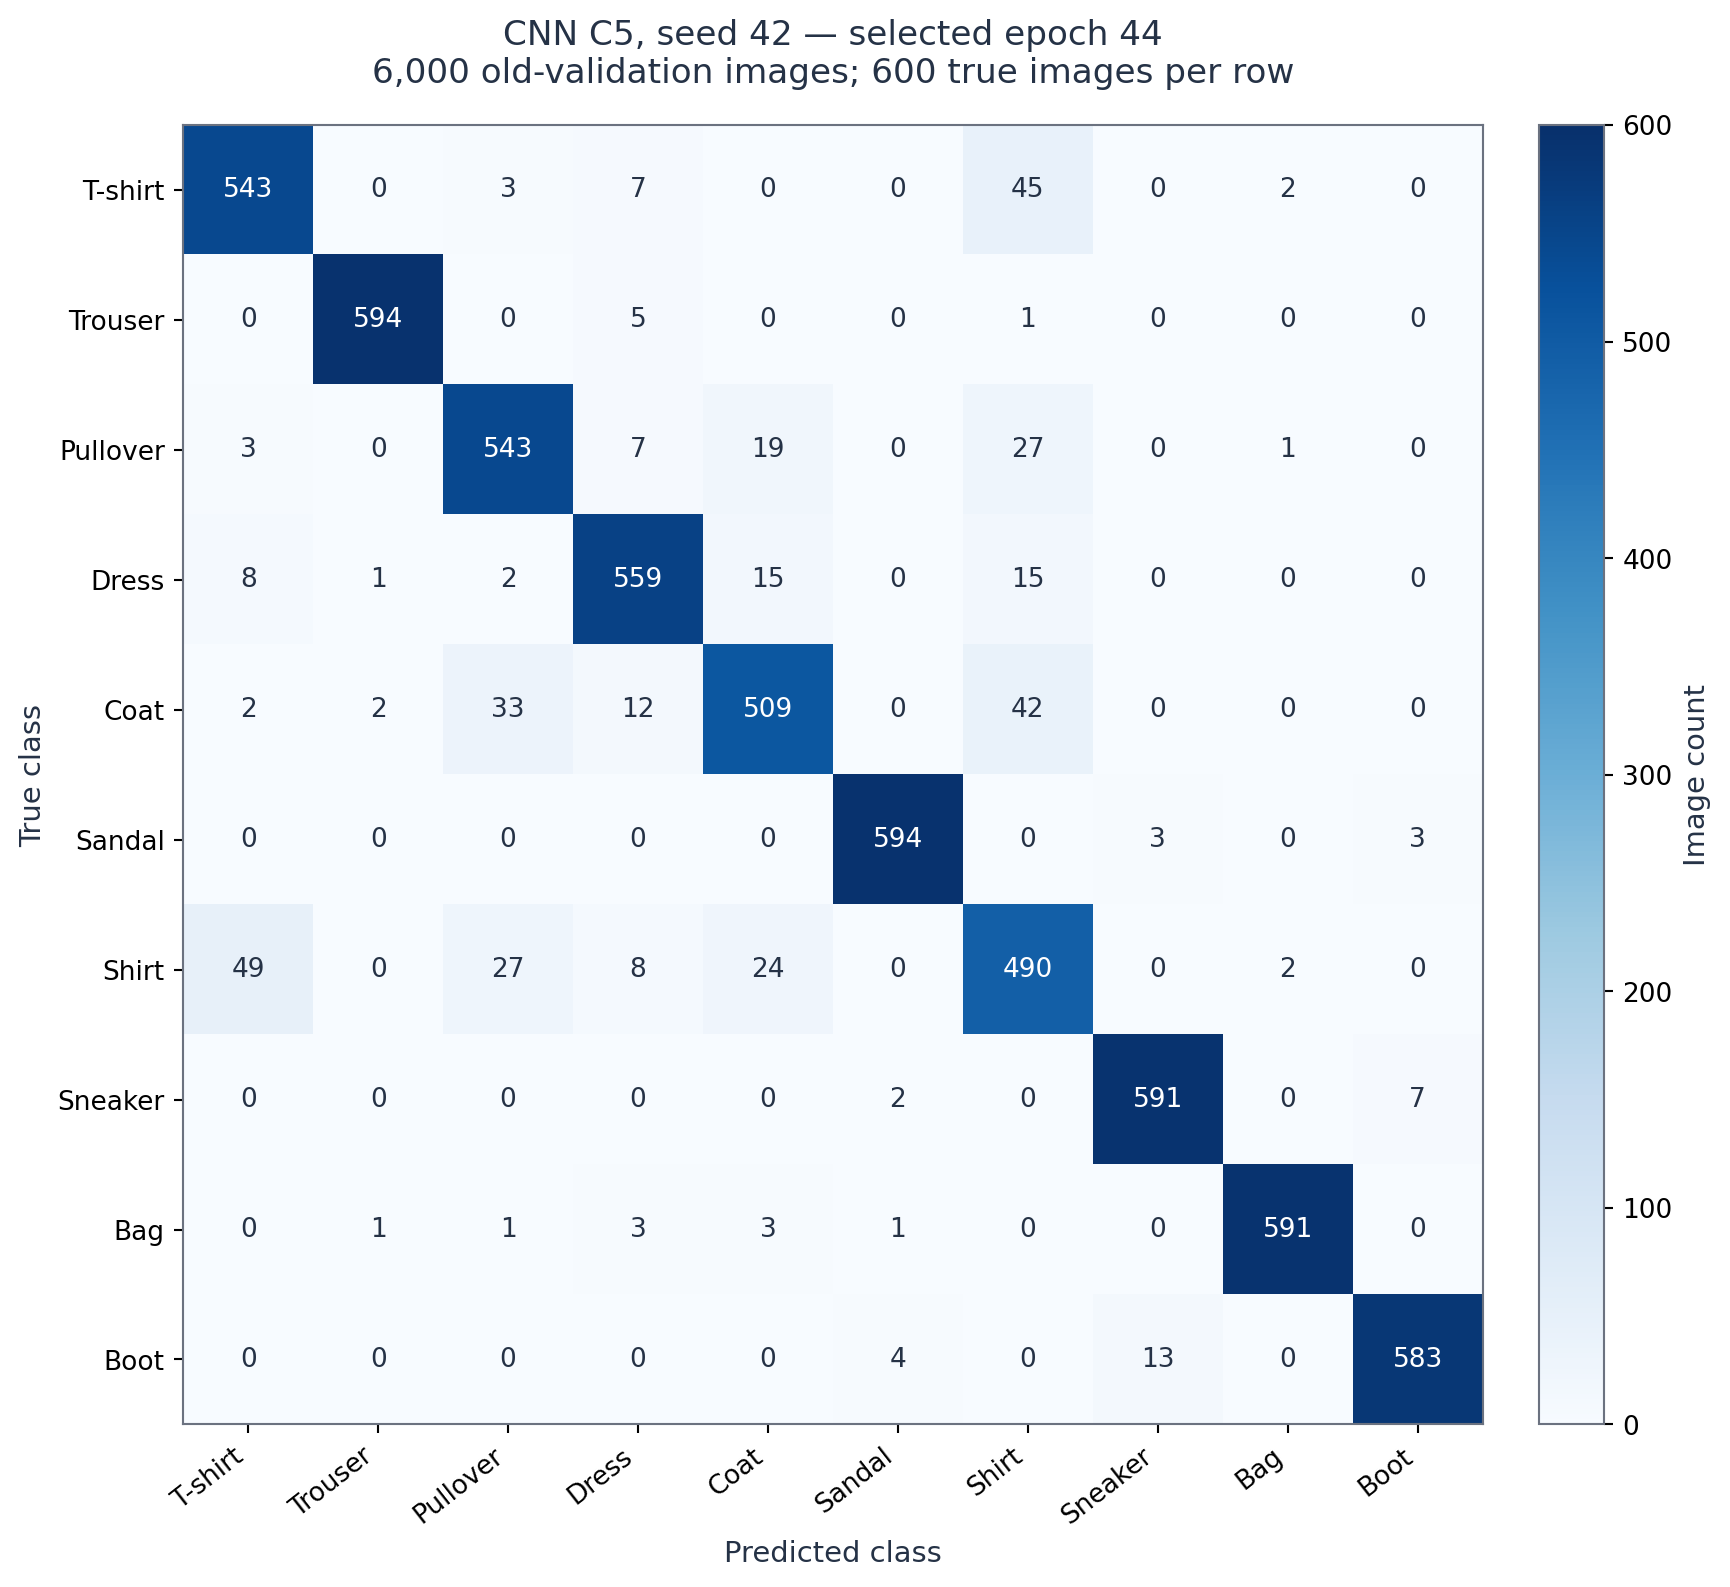
\includegraphics[width=0.84\linewidth]{figures/cnn_seed42_confusion.png}
\caption{CNN C5, seed 42, epoch 44, on old validation. Rows are true classes and columns are predicted classes. Each row contains 600 images; cells are integer prediction counts.}
\label{fig:confusion}
\end{figure}
The largest confusion is Shirt $\rightarrow$ T-shirt: 49/600 = 8.17\% of true shirts. T-shirt $\rightarrow$ Shirt: 45/600 = 7.50\%, and Coat $\rightarrow$ Shirt: 42/600 = 7.00\%. These rates use the true-class denominator, not all 6,000 images. Trouser and Sandal each have 594/600 correct predictions in this checkpoint, whereas Shirt has 490/600.

The errors are concentrated among upper-body garments rather than evenly spread across classes. A plausible explanation is overlapping shape and texture at low resolution. The matrix establishes the confusion pattern; the proposed visual mechanism remains an interpretation to check against examples or a controlled experiment.

\clearpage
\subsection{Concrete examples and class-level variation}

\begin{figure}[H]
\centering
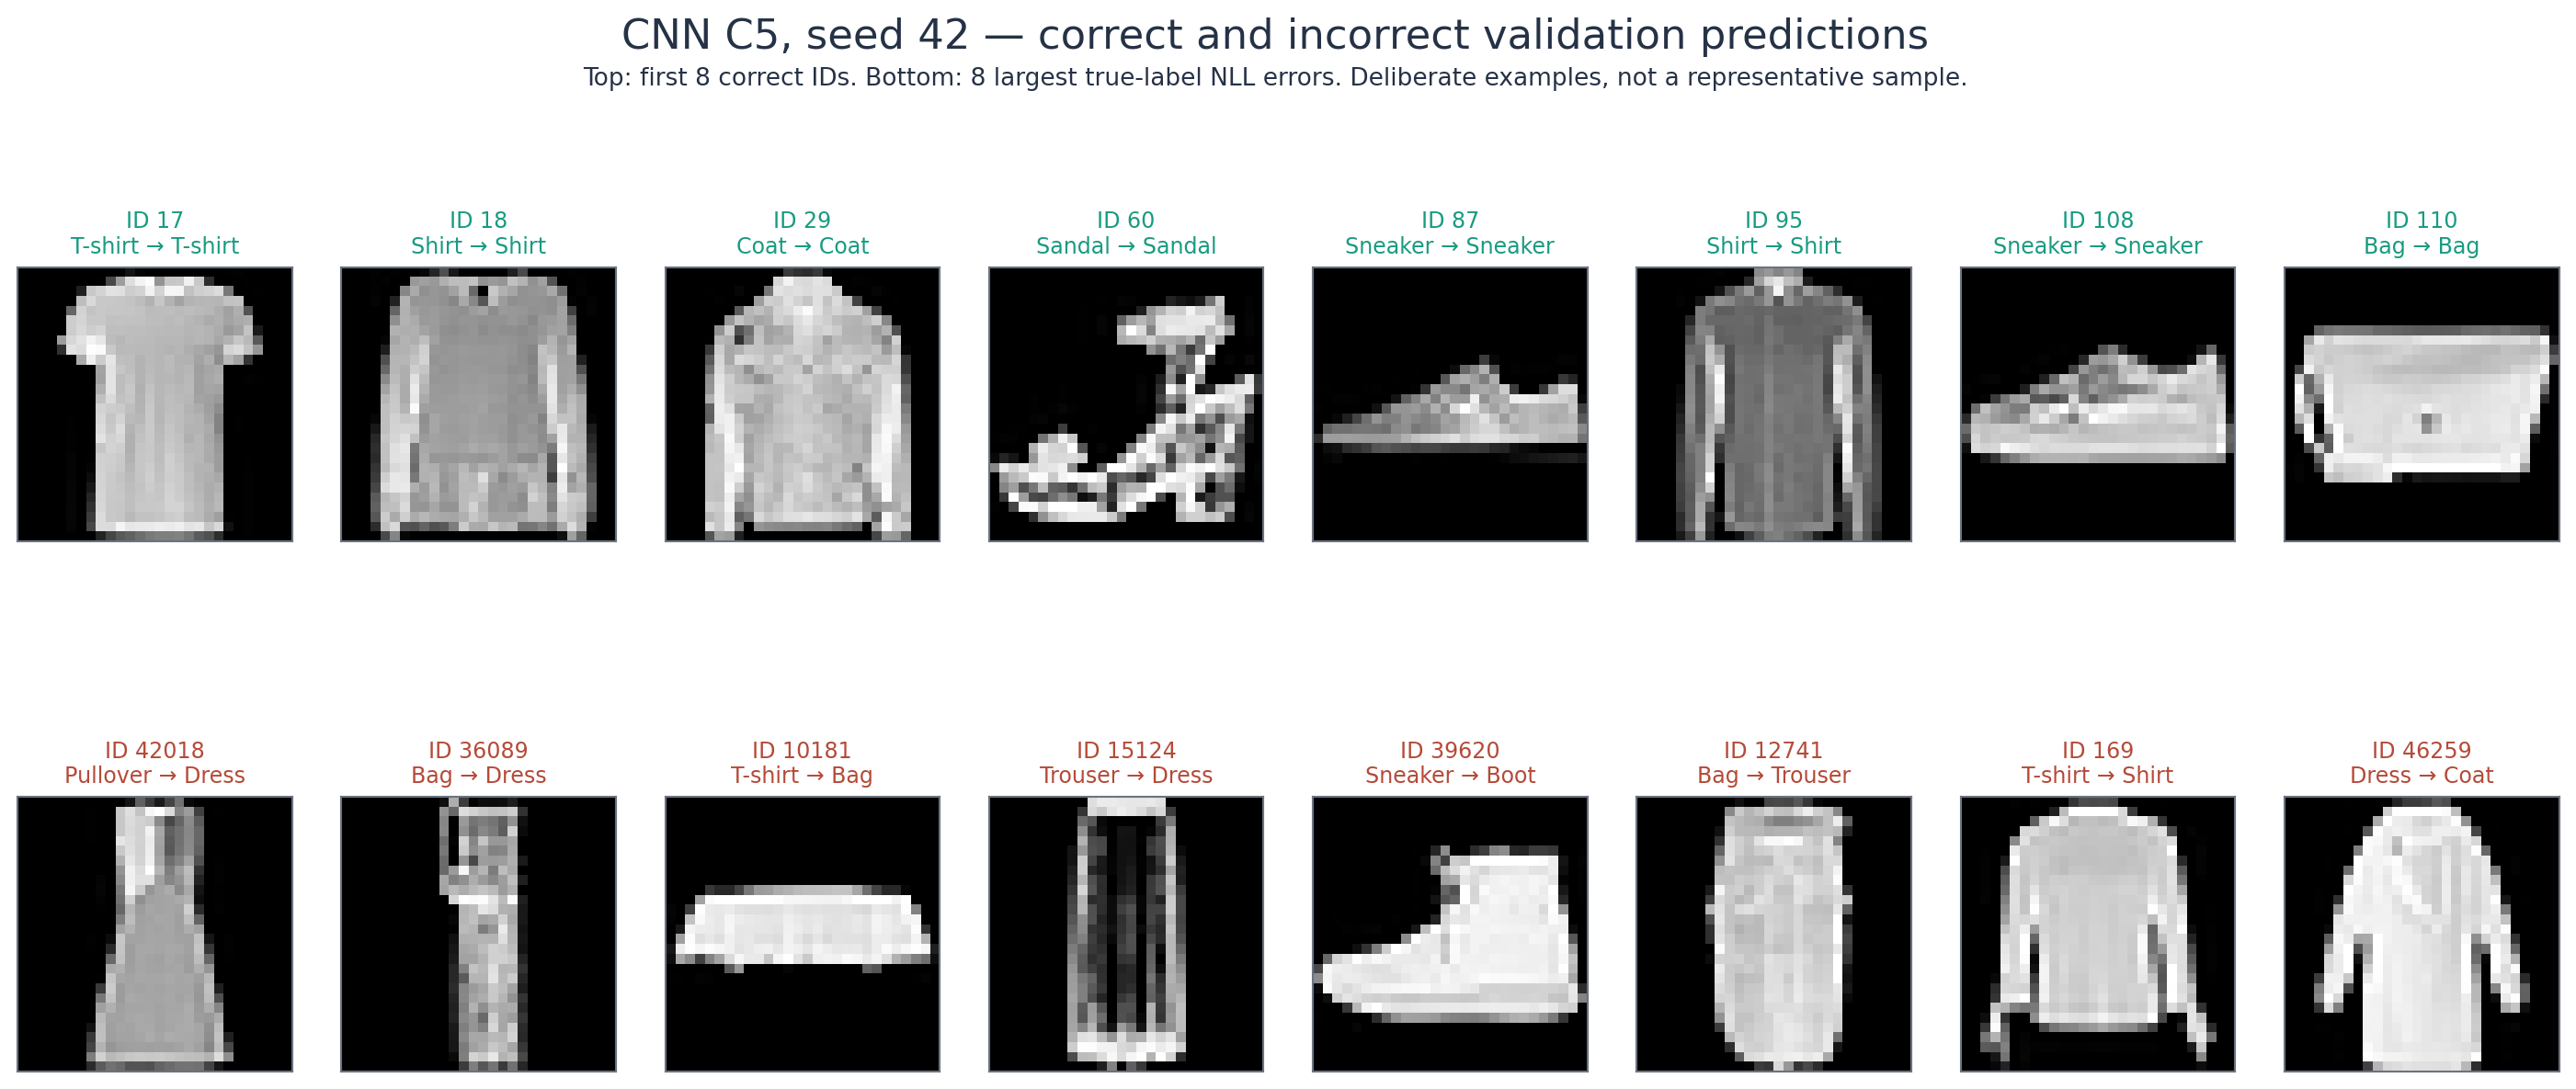
\includegraphics[width=\linewidth]{figures/cnn_seed42_examples.png}
\caption{Actual CNN C5 seed 42 predictions mapped back to official training-image IDs. Top: the first eight correct predictions by ID. Bottom: the eight errors with largest recorded true-label NLL. This deliberate selection illustrates failure cases and does not estimate their frequency.}
\label{fig:examples}
\end{figure}
Some selected errors have shapes that resemble the predicted class, including items labeled as bags or pullovers with unusual silhouettes. The supplied labels are retained. NLL ordering emphasizes errors to which the model assigns particularly unfavorable true-label probability, while the complete confusion matrix establishes the frequency of each error category.

The table below complements the single-seed image examples with CNN class F1 over all three final seeds. Its SD still describes training variation on the same validation images.

\begin{center}
\small
\begin{tabular}{lrr}
\toprule
Class & CNN class F1(\%) & Sample SD(pp) \\
\midrule
T-shirt/top & 90.12 & 0.59 \\
Trouser & 99.22 & 0.05 \\
Pullover & 89.53 & 0.29 \\
Dress & 93.01 & 0.08 \\
Coat & 87.61 & 0.57 \\
Sandal & 99.09 & 0.17 \\
Shirt & 80.15 & 0.43 \\
Sneaker & 97.70 & 0.26 \\
Bag & 98.78 & 0.05 \\
Ankle boot & 97.88 & 0.18 \\
\bottomrule
\end{tabular}
\end{center}
Shirt has the lowest mean class F1, about 80.15\%, despite the overall macro-F1 exceeding 93\%. The class-level results identify upper-body garment discrimination as the main remaining weakness. A targeted future comparison could test whether higher-resolution features or class-aware training improve these confusions while retaining the same evaluation protocol; those effects are not measured here.

\clearpage
\section{Efficiency and measured runtime}

\begin{figure}[H]
\centering
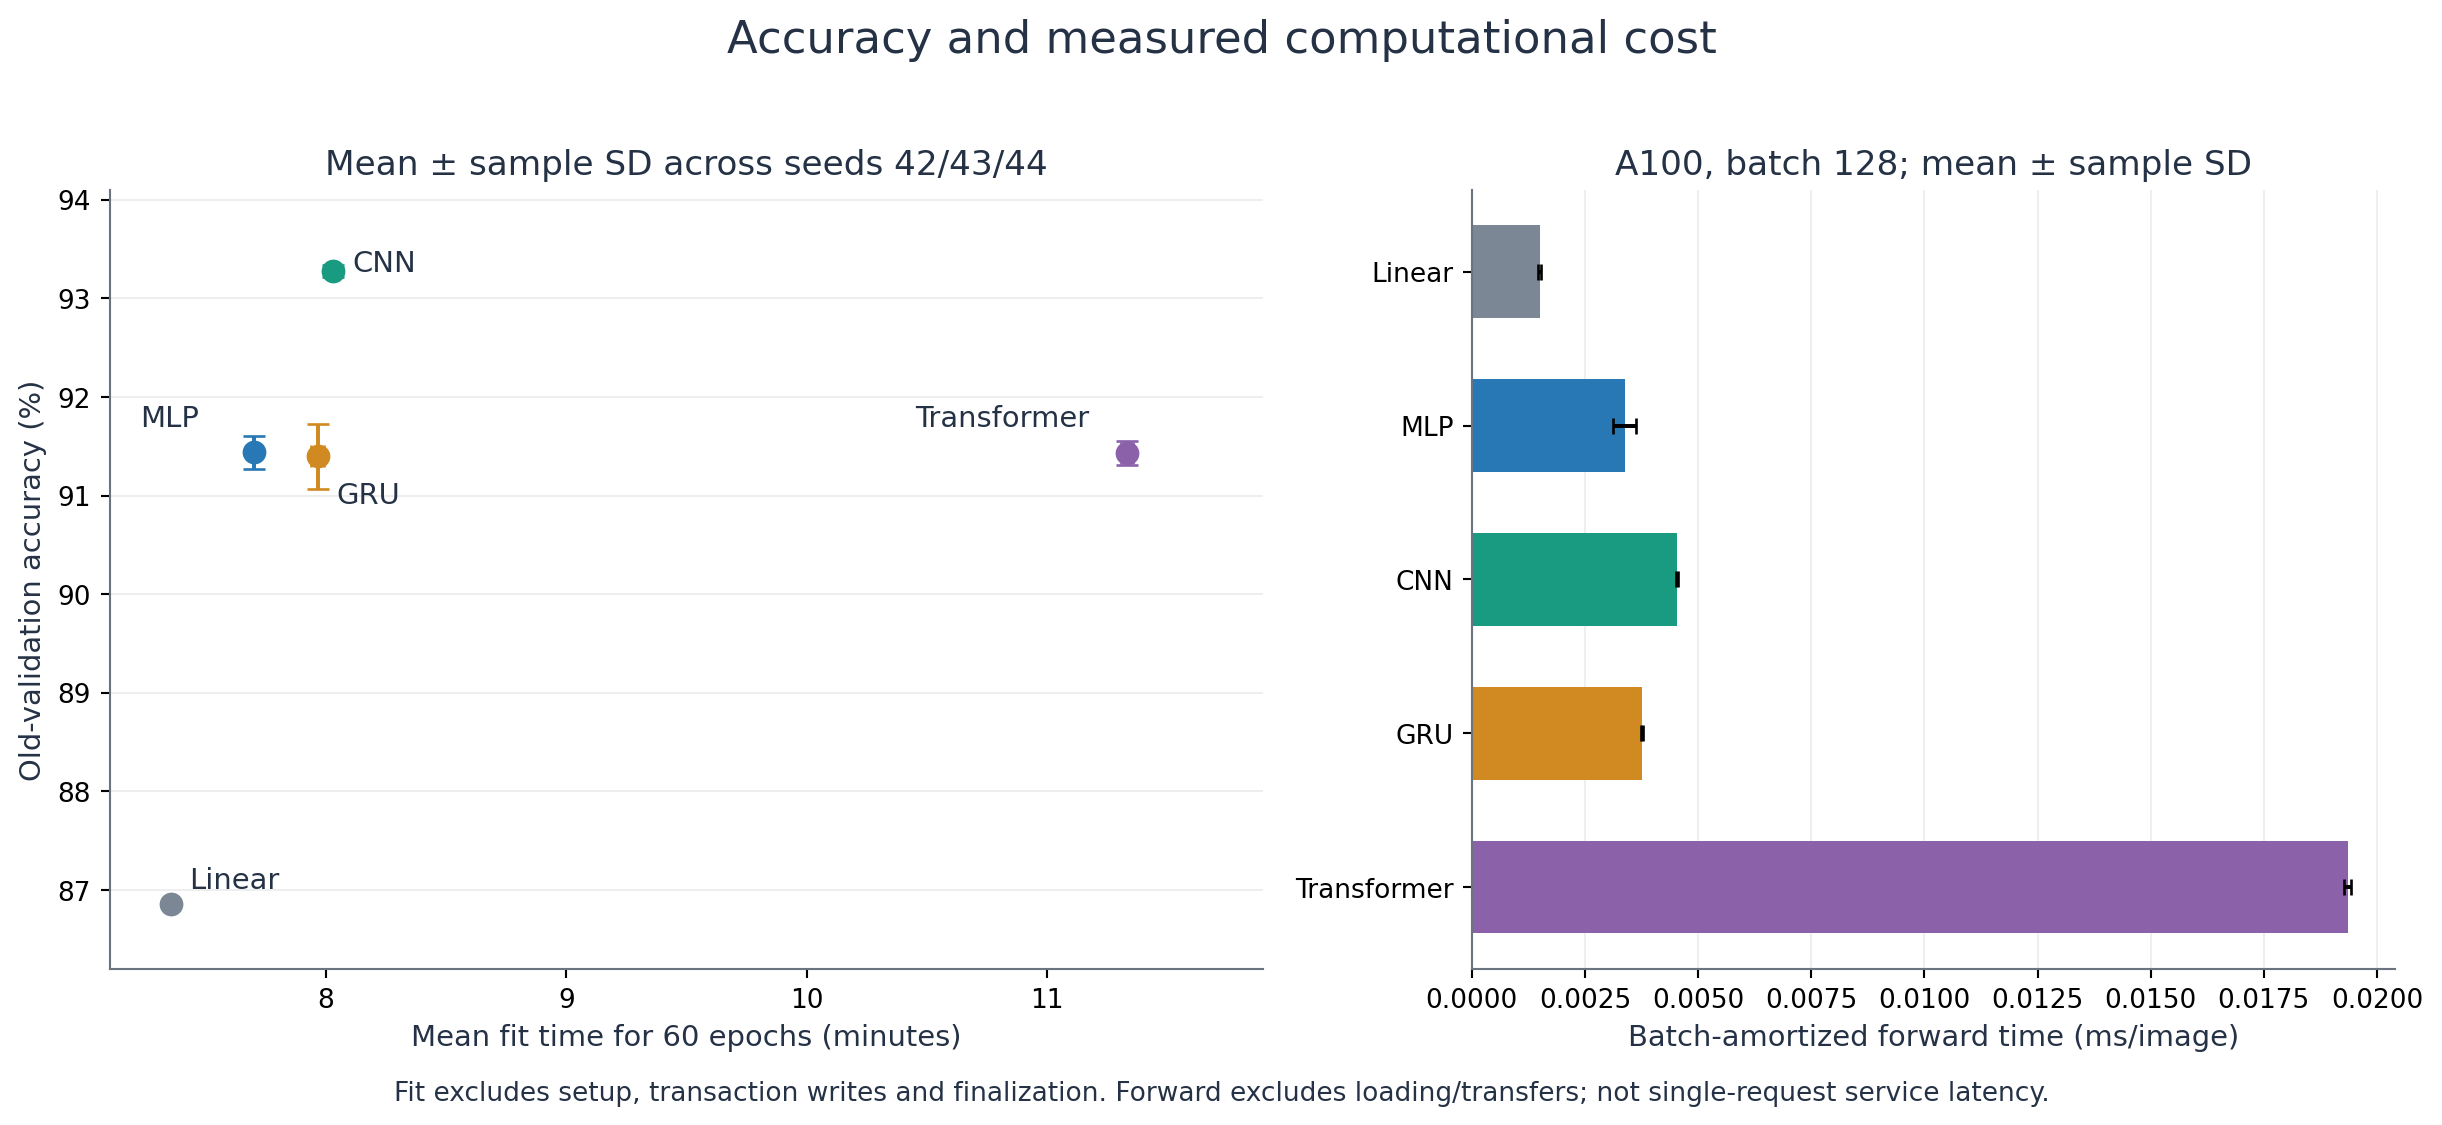
\includegraphics[width=\linewidth]{figures/accuracy_cost.png}
\caption{Final selected recipes: validation accuracy versus mean fit time, and measured batch-amortized forward time. Error bars are sample SD over three seeds. Fit timing and forward timing have different scopes; neither is an energy measurement.}
\label{fig:cost}
\end{figure}
\begin{center}
\small
\begin{tabular}{lrrr}
\toprule
Model & Parameters & Fit seconds & Forward ms/image \\
\midrule
Linear & 7,850 & $441.36 \pm 0.20$ & $0.00150 \pm 0.00003$ \\
MLP & 203,530 & $462.01 \pm 0.47$ & $0.00338 \pm 0.00026$ \\
CNN & 93,962 & $481.90 \pm 0.26$ & $0.00453 \pm 0.00003$ \\
GRU & 61,962 & $477.95 \pm 1.66$ & $0.00375 \pm 0.00002$ \\
Transformer & 274,954 & $679.87 \pm 1.46$ & $0.01935 \pm 0.00007$ \\
\bottomrule
\end{tabular}
\end{center}
\begin{center}
\small
\begin{tabular}{lrrr}
\toprule
Phase & Tasks & Fit minutes & Attempt minutes \\
\midrule
Discovery & 36 & 287.95 & 293.17 \\
Confirmation & 10 & 76.02 & 77.55 \\
Final & 15 & 127.15 & 129.62 \\
\bottomrule
\end{tabular}
\end{center}
The controller's recorded active time is about 8.34 hours. Completed-epoch fit time sums to about 8.19 hours; the sum of task-attempt wall timers is about 8.34 hours. Fit time includes training, validation and in-memory selection, while excluding setup, transaction writes and finalization. The controller clock excludes setup/smoke and may miss an abrupt unrecorded final tail. Their different boundaries account for the differences among these totals.

Forward timing uses A100 inputs already on the device, batch 128, ten warmup batches and 50 measured batches. Dividing batch time by 128 yields amortized milliseconds per image; it is not the latency of one independent service request. The Transformer has the largest parameter count and the highest measured forward cost. CNN combines the highest selected-validation score with 93,962 parameters, fewer than either MLP or Transformer. GRU uses fewer parameters than CNN but has lower mean F1. These are observed operating points, rather than a parameter- or compute-matched architecture experiment.

\clearpage
\section{Discussion and conclusion}
\subsection{What the experiments support}
The original fixed-budget test comparison favors the CNN among the five recorded checkpoints. The final exploratory study also gives CNN the highest validation macro-F1. Its image-specific local structure is consistent with this result, but the experiments do not establish inductive bias as the sole cause: architecture sizes, optimization behavior and training costs differ.

The search finds useful recipe candidates while preserving model size and input processing. The strongest matched-seed inner evidence is the MLP C7 improvement on both seeds. GRU C1 also improves on both, with a smaller margin. CNN's candidate improves on both inner seeds but the fresh-seed gain is much smaller. Linear's effect is small, and Transformer has mixed evidence. Selection and evidence strength therefore differ: the rule determines one recipe, while the paired margins quantify how much support that choice receives.

Checkpoint criterion changes interpretation. Macro-F1 directly targets class-wise classification balance, whereas CE evaluates true-label probabilities. The selected F1 checkpoint can have worse CE than a later or earlier CE-selected alternative. Keeping both artifacts makes that trade-off inspectable. The intended objective determines which checkpoint is appropriate; the recorded study prioritizes class-wise F1.

\subsection{Limits of the claims}
\begin{itemize}
\item The official test was observed before supplementary optimization. Final results are selected, previously seen validation results; no new blind test claim is made.
\item Only one inner split and one fresh confirmation seed are available. Discovery selection and checkpoint selection create additional optimism on those validation sets.
\item Three final training seeds do not measure split variance, population uncertainty or deployment robustness. Small sample SD is not a generalization guarantee.
\item The 61-fit phase did not include fresh final C0 anchors. Its historical CE-selected baseline differences cannot isolate recipe effects. Section~\ref{sec:matched-followup} reports the later matched C0 comparison under a shared checkpoint protocol.
\item The search is intentionally narrow: fixed architecture sizes, fixed optimizer families, no augmentation, no EMA/SWA and no ensemble. Their value remains an open empirical question.
\item Split-ID checks prevent sample-ID overlap; they do not establish absence of near-duplicate content or every possible dataset bias. Runtime is measured with explicit scopes, without energy or production-service measurements.
\end{itemize}

\subsection{Conclusion}
The project provides a reproducible comparison of five deep-learning model families, an original frozen test evaluation and a 61-task exploratory optimization study. The final CNN recipe achieves 93.308\% validation macro-F1 with 0.027 percentage-point seed SD. Across the three research questions, the evidence favors spatial convolution at the measured operating points, supports some recipe changes more consistently than others, and shows that the checkpoint objective changes which epoch is selected. The final 93.308\% Macro-F1 is a selected-validation result. Independent test performance of the optimized checkpoints remains unmeasured. The historical baseline comparison does not isolate HPO effects; the later matched study in Section~\ref{sec:matched-followup} addresses recipe versus checkpoint differences on the same old-validation images.
